\section{Modeling the Bridge Using mCRL2}
\label{sec:model}

With the requirements clearly stated, now the bridge can be modeled. In order to create a model that can be verified using $\mu$-calculus, the mCRL2 program can be used. The code for the model can be found in \ref{sec:mcrl} or the attached file \texttt{Bridge\_group7.mcrl2}.

When writing the code, we kept to the architecture from section \ref{sec:act} including three processes. The \emph{signs} process communicates with the \emph{barriers} process, which in turn communicates with the \emph{bridge} process. This leads to a linear structure of the model. The global actions consist of all possible commands that the bridge operator can send out, listed in table \ref{tab:allow}. Only the ones that are considered safe according to the safety layer are allowed. They turn out to be transitions to either the next state, the previous state or the same state (depicted as self loops). A screen of our current model is shown in figure \ref{fig:graph}.
%
\begin{table}[htb]%
\begin{tabular}{ll}
	\texttt{openBridge},& \texttt{closeBridge},\\
	\texttt{sendPre(on)},& \texttt{sendPre(off)},\\
	\texttt{sendStop(on)},& \texttt{sendStop(off)},\\
	\texttt{sendBar\_front(lift)},& \texttt{sendBar\_front(lower},\\
	\texttt{sendBar\_back(lift)},& \texttt{sendBar\_back(lower)},\\
	\texttt{sendLock(engaged)},& \texttt{sendLock(disengaged)},\\
	\texttt{sendDeck(up)},& \texttt{sendDeck(down).}\\
\end{tabular}
\caption{All possible user input to be expected at all times.}
\label{tab:allow}
\end{table}
%
\begin{figure}[htb]
\centering
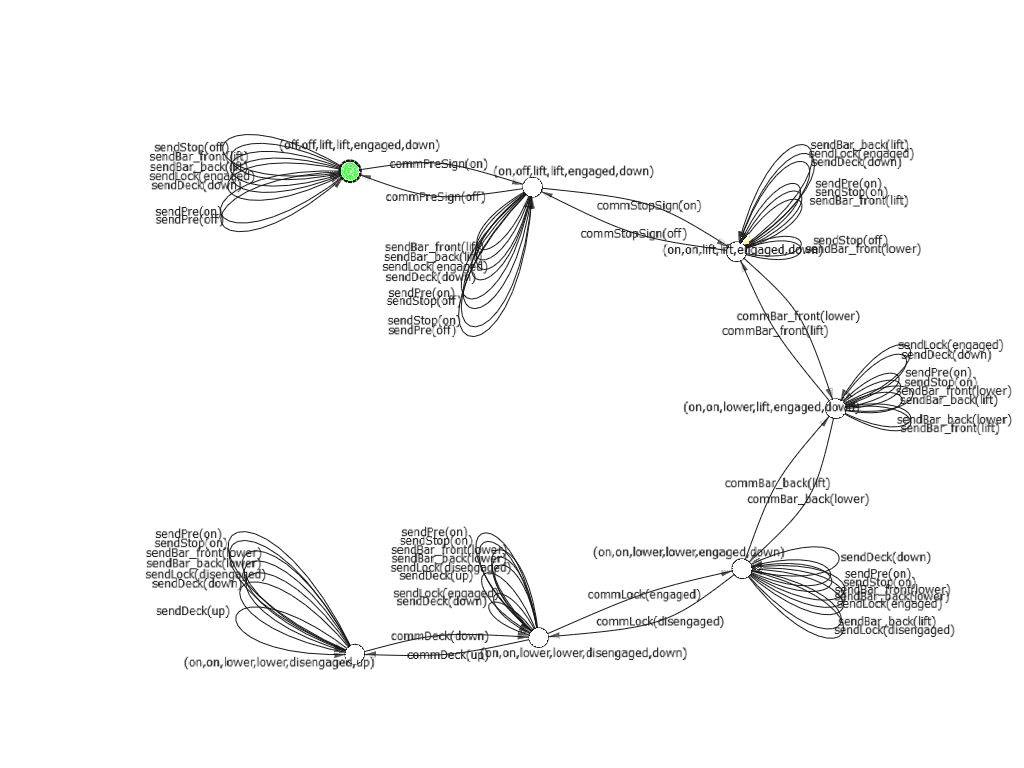
\includegraphics[width=\columnwidth]{Images/Bridge_allow_ltsgraph.png}
\caption{Graphical representation of the Bridge model.}%
\label{fig:graph}
\end{figure}%
%

\newpage